\section{Definitionsphase}

% Neurowissenschaftliche Grundlagen
\subsection{Wissenschaftliche Grundlagen}
\subsubsection{Lernen}
\subsubsection{Synapsen}
\subsubsection{Neuronen}
\subsubsection{Neuronales Netz}
\subsection{Technische Grundlagen}

\subsection{Pflichtenheft}
Das Pflichtenheft ist analog zum
\hyperref[sec:arbeitspaketplan]{Arbeitspaketplan} in diesem Dokument nicht
genauer beschrieben, sondern in Form eines Backlog auf
\href{https://studienarbeitlernapp.atlassian.net/jira/software/projects/LER/boards/1}{\underline{Jira}}\footnote{\href{https://studienarbeitlernapp.atlassian.net/jira/software/projects/LER/boards/1}{https://studienarbeitlernapp.atlassian.net/jira/software/projects/LER/boards/1}}
aufgeführt. Dort kann entweder der Reiter \gqq{Roadmap} oder der Reiter
\gqq{Board} aufgerufen werden.

\subsection{Use Case Diagramm}

\begin{figure}[H]
  \centering
  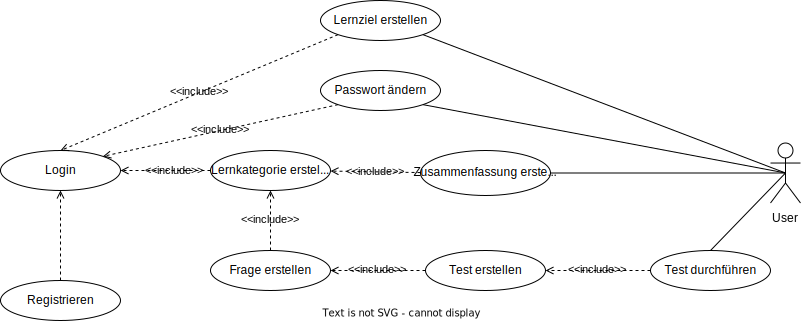
\includegraphics[width=1\textwidth]{images/diagramme/UseCase_Diagramm.png}
  \caption{Use Case Diagramm}
  \label{fig:UseCaseDiagramm}
\end{figure}
\newpage
\subsection{Use Case Beschreibung}

% Use Case Login
\begin{table}[h!]
  \begin{tabular}{p{0.2\textwidth}|p{0.74\textwidth}}
    \textbf{Name:}     & \textbf{Login}                                                                  \\ \hline
    Ziel:              & Anmelden mit bestehenden Logindaten in der App                                  \\ \hline
    Kategorie:         & Primär                                                                          \\ \hline
    Vorbedingung:      & Der Benutzer muss bereits einen Account erstellt haben                          \\ \hline
    Nachbedingung:     & Der Benutzer ist eingeloggt                                                     \\ \hline
    Fehlerfälle:       &
    \begin{minipage}[t]{\linewidth}
      Falsche Logindaten
      \strut
      \begin{itemize}
        \item Rückmeldung, dass falsche Zugangsdaten verwendet wurden
        \item Möglichkeit, das Kennwort über die E-Mail zurückzusetzen
      \end{itemize}
      Abbruch durch den Benutzer
      \begin{itemize}
        \item keine Zustandsänderung \strut
      \end{itemize}
    \end{minipage}                                                                       \\ \hline
    Akteure:           & User                                                                            \\ \hline
    Auslösendes Event: & Benutzer öffnet die App und klickt auf einloggen                                \\ \hline
    Beschreibung/
    Erweiterungen:     & Der Benutzer meldet sich an, um die verschiedenen Dienste der App zu verwenden  \\ \hline
    Alternativen:      & Benutzer kann sich registrieren, sofern die E-Mail nicht schon registriert ist. \\
  \end{tabular}
\end{table}
% Use Case Registrieren
\begin{table}[h!]
  \begin{tabular}{p{0.2\textwidth}|p{0.74\textwidth}}
    \textbf{Name:}     & \textbf{Registrieren}                                       \\ \hline
    Ziel:              & Anlegen eines neuen Accounts                                \\ \hline
    Kategorie:         & Primär                                                      \\ \hline
    Vorbedingung:      & E-Mail ist noch nicht mit einem anderen Account registriert \\ \hline
    Nachbedingung:     & Der Benutzer ist eingeloggt                                 \\ \hline
    Fehlerfälle:       &
    \begin{minipage}[t]{\linewidth}
      E-Mail bereits verwendet
      \strut
      \begin{itemize}
        \item Rückmeldung, dass E-Mail bereits verwendet wurde
      \end{itemize}
      Abbruch durch den Benutzer
      \begin{itemize}
        \item Keine Zustandsänderung
        \item Account wird nicht angelegt \strut
      \end{itemize}
    \end{minipage}                                                   \\ \hline
    Akteure:           & User                                                        \\ \hline
    Auslösendes Event: & Benutzer öffnet die App und klickt auf Registrieren.        \\ \hline
    Beschreibung/
    Erweiterungen:     & Ein Benutzer möchte einen neuen Account erstellen.          \\ \hline
    Alternativen:      & Login mit bestehendem Account.                              \\
  \end{tabular}
\end{table}
% Use Case Lernziel erstellen
\begin{table}[h!]
  \begin{tabular}{p{0.2\textwidth}|p{0.74\textwidth}}
    \textbf{Name:}     & \textbf{Lernziel erstellen}                                                                                                                                                \\ \hline
    Ziel:              & Anlegen eines neuen Lernziels                                                                                                                                              \\ \hline
    Kategorie:         & Primär                                                                                                                                                                     \\ \hline
    Vorbedingung:      &
    \begin{minipage}[t]{\linewidth}
      \strut
      \begin{itemize}
        \item User musss eingeloggt sein
        \item Lernziel mit gleichem Namen ist noch nicht erstellt \strut
      \end{itemize}
    \end{minipage}                                                                                                                                                                  \\ \hline
    Nachbedingung:     & Lernziel ist erstellt                                                                                                                                                      \\ \hline
    Fehlerfälle:       &
    \begin{minipage}[t]{\linewidth}
      Lernziel mit gleichem Namen existiert bereits
      \strut
      \begin{itemize}
        \item Rückmeldung, dass dieses Lernziel bereits existiert
      \end{itemize}
      Abbruch durch den Benutzer
      \begin{itemize}
        \item keine Zustandsänderung
        \item Lernziel wird nicht angelegt \strut
      \end{itemize}
    \end{minipage}                                                                                                                                                    \\ \hline
    Akteure:           & User                                                                                                                                                                       \\ \hline
    Auslösendes Event: & Benutzer öffnet Lernziel Reiter und klickt auf \gqq{Lernziel erstellen}                                                                                                    \\ \hline
    Beschreibung/
    Erweiterungen:     & Durch das Ausfüllen der Eingabefelder und anschließendes bestätigen, kann der User ein Lernziel erstellen. Aus sämtlichen Lernzielen wird daraufhin ein Lernplan erstellt. \\ \hline
    Alternativen:      &                                                                                                                                                                            \\
  \end{tabular}
\end{table}
% Use Case Lernkategorie erstellen
\begin{table}[H]
  \begin{tabular}{p{0.2\textwidth}|p{0.74\textwidth}}
    \textbf{Name:}     & \textbf{Lernkategorie erstellen}                                                                                                                                                                         \\ \hline
    Ziel:              & Anlegen einer neuen Lernkategorie                                                                                                                                                                   \\ \hline
    Kategorie:         & Primär                                                                                                                                                                                              \\ \hline
    Vorbedingung:      &
    \begin{minipage}[t]{\linewidth}
      \strut
      \begin{itemize}
        \item User musss eingeloggt sein
        \item Lernkategorie mit gleichem Namen ist noch nicht erstellt \strut
      \end{itemize}
    \end{minipage}                                                                                                                                                                                           \\ \hline
    Nachbedingung:     & Lernkategorie ist erstellt                                                                                                                                                                          \\ \hline
    Fehlerfälle:       &
    \begin{minipage}[t]{\linewidth}
      Lernkategorie mit gleichem Namen existiert bereits
      \strut
      \begin{itemize}
        \item Rückmeldung, dass diese Lernkategorie bereits existiert
      \end{itemize}
      Abbruch durch den Benutzer
      \begin{itemize}
        \item keine Zustandsänderung
        \item Lernkategorie wird nicht angelegt \strut
      \end{itemize}
    \end{minipage}                                                                                                                                                                        \\ \hline
    Akteure:           & User                                                                                                                                                                                                \\ \hline
    Auslösendes Event: & Benutzer öffnet Lernkategorie Reiter und klickt auf \gqq{Lernkategorie erstellen}                                                                                                                   \\ \hline
    Beschreibung/
    Erweiterungen:     & Durch das Ausfüllen der Eingabefelder und anschließendes bestätigen, kann der User eine Lernkategorie erstellen. In einer Lernkategorie können Zusammenfassungen, Fragen und Tests erstellt werden. \\ \hline
    Alternativen:      &                                                                                                                                                                                                     \\
  \end{tabular}
\end{table}
% Use Case Zusammenfassung erstellen
\begin{table}[h!]
  \begin{tabular}{p{0.2\textwidth}|p{0.74\textwidth}}
    \textbf{Name:}     & \textbf{Zusammenfassung erstellen}                                                                                                                                                          \\ \hline
    Ziel:              & Anlegen einer neuen Zusammenfassung                                                                                                                                                         \\ \hline
    Kategorie:         & Primär                                                                                                                                                                                      \\ \hline
    Vorbedingung:      &
    \begin{minipage}[t]{\linewidth}
      \strut
      \begin{itemize}
        \item User musss eingeloggt sein
        \item Zusammenfassung mit gleichem Namen ist noch nicht in der gleichen Lernkategorie
              erstellt \strut
      \end{itemize}
    \end{minipage}                                                                                                                                                                                   \\ \hline
    Nachbedingung:     & Zusammenfassung für Lernkategorie ist erstellt                                                                                                                                              \\ \hline
    Fehlerfälle:       &
    \begin{minipage}[t]{\linewidth}
      Zusammenfassung mit gleichem Namen existiert bereits in dieser Lernkategorie
      \strut
      \begin{itemize}
        \item Rückmeldung, dass diese Zusammenfassung bereits existiert
      \end{itemize}
      Abbruch durch den Benutzer
      \begin{itemize}
        \item keine Zustandsänderung
        \item Zusammenfassung wird nicht angelegt \strut
      \end{itemize}
    \end{minipage}                                                                                                                                      \\ \hline
    Akteure:           & User                                                                                                                                                                                        \\ \hline
    Auslösendes Event: & Benutzer öffnet eine Lernkategorie, klickt auf \gqq{Zusammenfassungen} und danach auf \gqq{Zusammenfassung erstellen}                                                                       \\ \hline
    Beschreibung/
    Erweiterungen:     & Durch das Ausfüllen der Eingabefelder und anschließendes bestätigen, kann der User eine Zusammenfassung erstellen. In einer Zusammenfassung können Inhalte eingefügt und formatiert werden. \\ \hline
    Alternativen:      &                                                                                                                                                                                             \\
  \end{tabular}
\end{table}
% Use Case Frage erstellen
\begin{table}[H]
  \begin{tabular}{p{0.2\textwidth}|p{0.74\textwidth}}
    \textbf{Name:}     & \textbf{Frage erstellen}                                                                                                                                                                                                                                               \\ \hline
    Ziel:              & Anlegen einer neuen Frage                                                                                                                                                                                                                                              \\ \hline
    Kategorie:         & Primär                                                                                                                                                                                                                                                                 \\ \hline
    Vorbedingung:      &
    \begin{minipage}[t]{\linewidth}
      \strut
      \begin{itemize}
        \item User musss eingeloggt sein
        \item Frage mit gleichem Index ist noch nicht in der gleichen Lernkategorie erstellt
              \strut
      \end{itemize}
    \end{minipage}                                                                                                                                                                                                                                                              \\ \hline
    Nachbedingung:     & Frage für Lernkategorie ist erstellt                                                                                                                                                                                                                                   \\ \hline
    Fehlerfälle:       &
    \begin{minipage}[t]{\linewidth}
      Frage mit gleichem Namen existiert bereits in dieser Lernkategorie
      \strut
      \begin{itemize}
        \item Rückmeldung, dass Frage mit gleicher Bezeichnung bereits existiert
      \end{itemize}
      Abbruch durch den Benutzer
      \begin{itemize}
        \item keine Zustandsänderung
        \item Frage wird nicht angelegt \strut
      \end{itemize}
    \end{minipage}                                                                                                                                                                                                                           \\ \hline
    Akteure:           & User                                                                                                                                                                                                                                                                   \\ \hline
    Auslösendes Event: & Benutzer öffnet eine Lernkategorie, klickt auf \gqq{Tests / Fragen} und danach auf \gqq{Frage erstellen}                                                                                                                                                               \\ \hline
    Beschreibung/
    Erweiterungen:     & Durch das Ausfüllen der Eingabefelder und anschließendes bestätigen, kann der User eine Frage erstellen. Eine Frage kann unterschiedliche Vorlagen (beispielsweise Karteikarte) besitzen, jedoch gibt es immer eine Meldung (Text der Frage) und eine gültige Antwort. \\ \hline
    Alternativen:      &                                                                                                                                                                                                                                                                        \\
  \end{tabular}
\end{table}
% Use Case Test erstellen
\begin{table}[H]
  \begin{tabular}{p{0.2\textwidth}|p{0.74\textwidth}}
    \textbf{Name:}     & \textbf{Test erstellen}                                                                                                                                                                                                                                                                           \\ \hline
    Ziel:              & Anlegen eines neuen Tests                                                                                                                                                                                                                                                                         \\ \hline
    Kategorie:         & Primär                                                                                                                                                                                                                                                                                            \\ \hline
    Vorbedingung:      &
    \begin{minipage}[t]{\linewidth}
      \strut
      \begin{itemize}
        \item User musss eingeloggt sein
        \item Test mit gleichem Namen ist noch nicht in der gleichen Lernkategorie erstellt
              \strut
      \end{itemize}
    \end{minipage}                                                                                                                                                                                                                                                                                         \\ \hline
    Nachbedingung:     & Test für Lernkategorie ist erstellt                                                                                                                                                                                                                                                               \\ \hline
    Fehlerfälle:       &
    \begin{minipage}[t]{\linewidth}
      Test mit gleichem Namen existiert bereits in dieser Lernkategorie
      \strut
      \begin{itemize}
        \item Rückmeldung, dass Test mit gleicher Bezeichnung bereits existiert
      \end{itemize}
      Abbruch durch den Benutzer
      \begin{itemize}
        \item keine Zustandsänderung
        \item Test wird nicht angelegt \strut
      \end{itemize}
    \end{minipage}                                                                                                                                                                                                                                                       \\ \hline
    Akteure:           & User                                                                                                                                                                                                                                                                                              \\ \hline
    Auslösendes Event: & Benutzer öffnet eine Lernkategorie, klickt auf \gqq{Tests / Fragen} und danach auf \gqq{Test erstellen}                                                                                                                                                                                           \\ \hline
    Beschreibung/
    Erweiterungen:     & Durch das Ausfüllen der Eingabefelder und anschließendes bestätigen, kann der User einen Test erstellen. Eine Test kann mehrere Fragen besitzen. Wenn ein Test gestartet wird, bekommt der User nach abschließen des Tests eine Meldung, wie viele und welche Fragen er richtig beantwortet hast. \\ \hline
    Alternativen:      &                                                                                                                                                                                                                                                                                                   \\
  \end{tabular}
\end{table}
\newpage

\subsection{Datenbankstruktur}
\subsubsection{Datenbankmodell}
\begin{figure}[H]
  \centering
  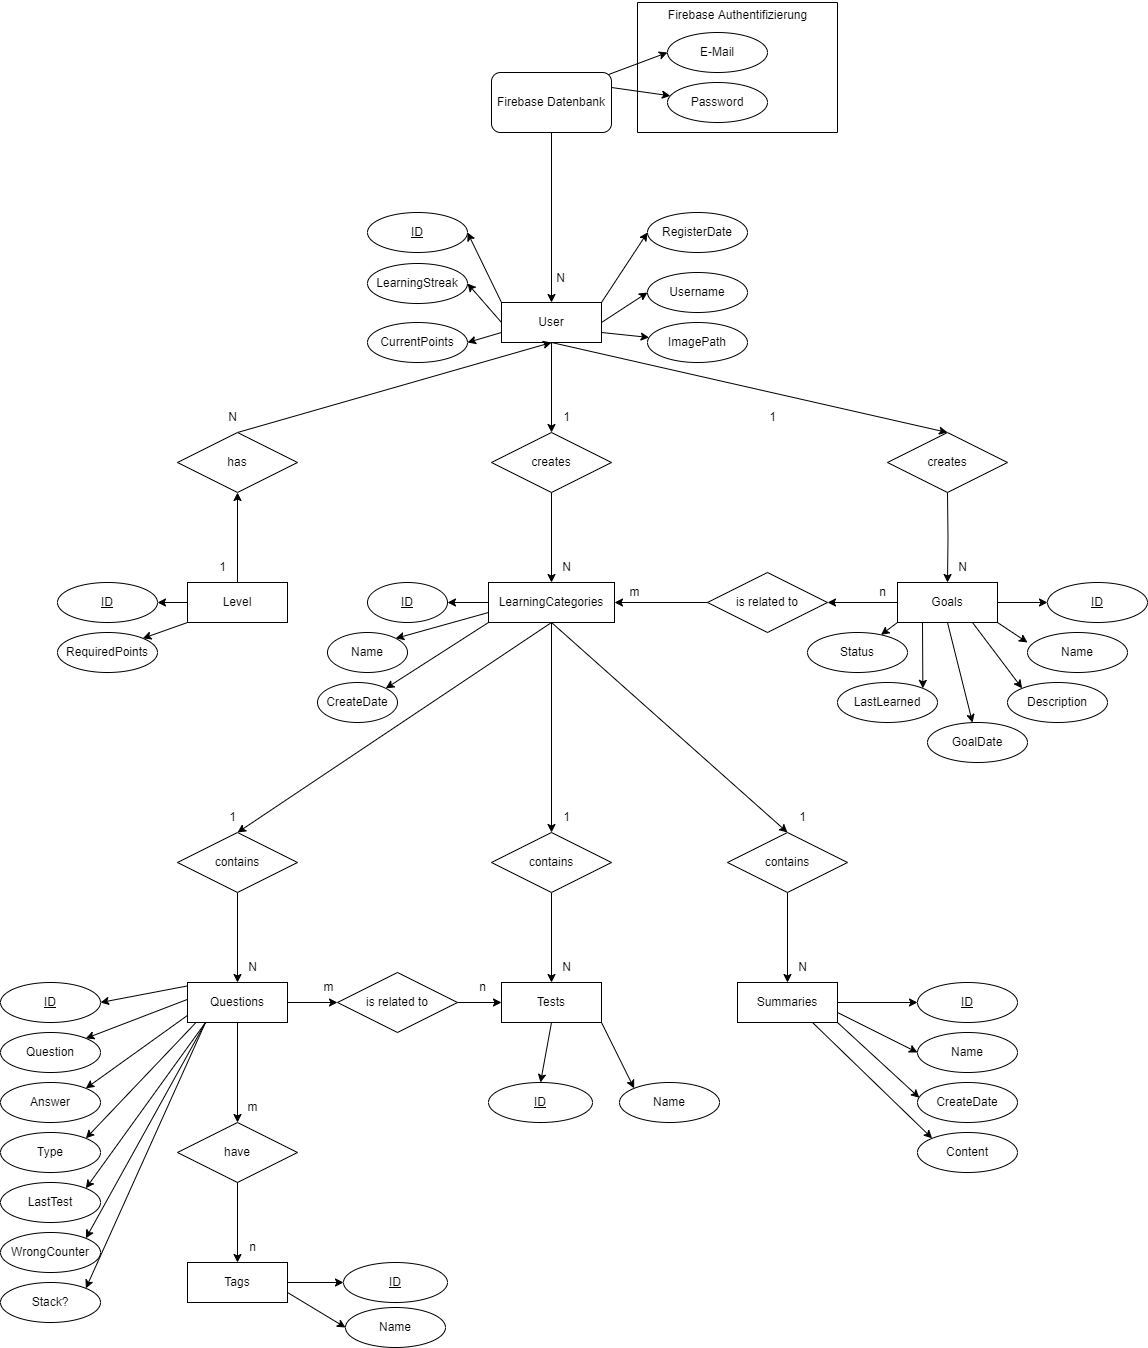
\includegraphics[width=1\textwidth]{images/LearnAheadDatenbankstruktur.png}
  \caption{LearnAhead Datenbankstruktur}
  \label{fig:LearnAheadDatenbankstruktur}
\end{figure}\noindent
\subsubsection{Data Dictionary}
\underline{\textbf{User}}
\begin{table}[H]
  \centering
  \resizebox{\columnwidth}{!}{%
    \begin{tabular}{c|c|c|c|c|c|l}
      \textbf{Attribut}  &
      \textbf{Datentyp}  &
      \textbf{Länge}     &
      \textbf{Null}      &
      \textbf{Default}   &
      \textbf{Schlüssel} &
      \textbf{Beschreibung}                                                                                                                                                         \\ \hline
      ID                 &
      string             &
      -                  &
      Nein               &
      -                  &
      P                  &
      \\ \hline
      Username           &
      string             &
      -                  &
      Nein               &
      -                  &
      -                  &
      Der Benutzername des Nutzers                                                                                                                                                  \\ \hline
      E-Mail             &
      string             &
      -                  &
      Nein               &
      -                  &
      -                  &
      Die E-Mail-Adresse des Nutzers                                                                                                                                                \\ \hline
      Password           &
      string             &
      -                  &
      Nein               &
      -                  &
      -                  &
      Das Passwort des Nutzers                                                                                                                                                      \\ \hline
      ProfileImageURL    &
      string             &
      -                  &
      Ja                 &
      Null               &
      -                  &
      \begin{tabular}[c]{@{}l@{}}Der Link des Profilbilds welches\\ im Firebase Storage gespeichert\\ ist\end{tabular}                                                              \\ \hline
      RegisterDate       &
      timestamp          &
      -                  &
      Nein               &
      -                  &
      -                  &
      \begin{tabular}[c]{@{}l@{}}Das Datum an dem sich der \\ Nutzer registriert hat.\end{tabular}                                                                                  \\ \hline
      LearningStreak     &
      number             &
      -                  &
      Ja                 &
      0                  &
      -                  &
      \begin{tabular}[c]{@{}l@{}}Dies gibt die Anzahl an, wie viele\\ Tage der Nutzer aufeinander \\ gelernt hat.\end{tabular}                                                      \\ \hline
      AchievedGoals      &
      number             &
      -                  &
      Ja                 &
      0                  &
      -                  &
      \begin{tabular}[c]{@{}l@{}}Dies gibt die Anzahl an, wie viele\\ Lernziel der Nutzer erreicht hat.\end{tabular}                                                                \\ \hline
      CurrentPoints      &
      number             &
      -                  &
      Ja                 &
      0                  &
      -                  &
      \begin{tabular}[c]{@{}l@{}}Die aktuelle Level Punkte des\\ Nutzers\end{tabular}                                                                                               \\ \hline
      LearningCategories &
      map                &
      -                  &
      Ja                 &
      Null               &
      -                  &
      \begin{tabular}[c]{@{}l@{}}Dies ist eine gemappte Liste zu\\ der Tabelle LearningCategories, \\ wo alle Lernkategorien drin sind,\\ die der Nutzer erstellt hat.\end{tabular} \\ \hline
      Goals              &
      map                &
      -                  &
      Ja                 &
      Null               &
      -                  &
      \begin{tabular}[c]{@{}l@{}}Dies ist eine gemappte Liste zu \\ der Tabelle Goals, wo alle\\ Lernziele drin sind, die der\\ Nutzer erstellt hat.\end{tabular}
    \end{tabular}%
  }
\end{table}
\underline{\textbf{Level}}
\begin{table}[H]
  \centering
  \resizebox{\columnwidth}{!}{%
  \begin{tabular}{c|c|c|c|c|c|l}
  \textbf{Attribut} &
    \textbf{Datentyp} &
    \textbf{Länge} &
    \textbf{Null} &
    \textbf{Default} &
    \textbf{Schlüssel} &
    \textbf{Beschreibung} \\ \hline
  ID &
    string &
    - &
    Nein &
    - &
    P &
     \\ \hline
  RequiredPoints & number & - & Nein & - & - & \begin{tabular}[c]{@{}l@{}}Dies gibt die benötigten\\ Punkte für das spezielle\\ Level an\end{tabular} \\ \hline
  Level &
    number &
    - &
    Nein &
    - &
    - &
    \begin{tabular}[c]{@{}l@{}}Dies gibt das spezielle \\ Level anhand der Punkte an\end{tabular}
  \end{tabular}%
  }
  \end{table}
\newpage
\underline{\textbf{Goal}}
\begin{table}[H]
  \centering
  \resizebox{\columnwidth}{!}{%
    \begin{tabular}{c|c|c|c|c|c|l}
      \textbf{Attribut}                                          &
      \textbf{Datentyp}                                          &
      \textbf{Länge}                                             &
      \textbf{Null}                                              &
      \textbf{Default}                                           &
      \textbf{Schlüssel}                                         &
      \textbf{Beschreibung}                                                                                                                                       \\ \hline
      ID                                                         &
      string                                                     &
      -                                                          &
      Nein                                                       &
      -                                                          &
      P                                                          &
      \\ \hline
      Name                                                       &
      string                                                     &
      -                                                          &
      Nein                                                       &
      -                                                          &
      -                                                          &
      Der Name des Lernziels                                                                                                                                      \\ \hline
      Description                                                &
      string                                                     &
      -                                                          &
      Ja                                                         &
      Null                                                       &
      -                                                          &
      \begin{tabular}[c]{@{}l@{}}Dies soll als Beschreibung des\\ Lernziels gelten. Hier können\\ z.B. die relevanten Themen\\ aufgelistet werden.\end{tabular}   \\ \hline
      Status                                                     &
      string                                                     &
      -                                                          &
      Ja                                                         &
      ToDo                                                       &
      -                                                          &
      \begin{tabular}[c]{@{}l@{}}Dies gibt den aktuellen Status\\ des Lernziels an.\\ Es gibt die folgende Status:\\ - ToDo\\ - In Progress\\ - Done\end{tabular} \\ \hline
      StartDate                                                  &
      timestamp                                                  &
      -                                                          &
      Ja                                                         &
      \begin{tabular}[c]{@{}c@{}}Server\\ Timestamp\end{tabular} &
      -                                                          &
      \begin{tabular}[c]{@{}l@{}}Dies gibt an, wann das \\ Lernziel startet\end{tabular}                                                                          \\ \hline
      EndDate                                                    &
      timestamp                                                  &
      -                                                          &
      Nein                                                       &
      -                                                          &
      -                                                          &
      \begin{tabular}[c]{@{}l@{}}Dies gibt an, bis wann das\\ Lernziel abgeschlossen sein\\ soll\end{tabular}                                                     \\ \hline
      LastLearned                                                &
      timestamp                                                  &
      -                                                          &
      Ja                                                         &
      Null                                                       &
      -                                                          &
      \begin{tabular}[c]{@{}l@{}}Dies gibt, wann das Lernziel\\ das letzte mal gelernt wurde.\end{tabular}
    \end{tabular}%
  }
\end{table}
\newpage
% Data Dicitonary Learning Category Table
\underline{\textbf{LearningCategory}}
\begin{table}[H]
  \centering
  \resizebox{\columnwidth}{!}{%
    \begin{tabular}{c|c|c|c|c|c|l}
      \textbf{Attribut}                                          &
      \textbf{Datentyp}                                          &
      \textbf{Länge}                                             &
      \textbf{Null}                                              &
      \textbf{Default}                                           &
      \textbf{Schlüssel}                                         &
      \textbf{Beschreibung}                                                                                                                                                \\ \hline
      ID                                                         &
      string                                                     &
      -                                                          &
      Nein                                                       &
      -                                                          &
      P                                                          &
      \\ \hline
      Name                                                       &
      string                                                     &
      -                                                          &
      Nein                                                       &
      -                                                          &
      -                                                          &
      Der Name der Lernkategorie                                                                                                                                           \\ \hline
      CreateDate                                                 &
      timestamp                                                  &
      -                                                          &
      Ja                                                         &
      \begin{tabular}[c]{@{}c@{}}Server\\ Timestamp\end{tabular} &
      -                                                          &
      \begin{tabular}[c]{@{}l@{}}Dies gibt an, wann die \\ Lernkategorie erstellt wurde\end{tabular}                                                                       \\ \hline
      Goals                                                      &
      map                                                        &
      -                                                          &
      Ja                                                         &
      Null                                                       &
      -                                                          &
      \begin{tabular}[c]{@{}l@{}}Dies ist eine gemappte Liste zu\\ der Tabelle Goal,\\ wo alle Lernziele drin sind,\\ die der Nutzer erstellt hat.\end{tabular}            \\ \hline
      Questions                                                  &
      map                                                        &
      -                                                          &
      Ja                                                         &
      Null                                                       &
      -                                                          &
      \begin{tabular}[c]{@{}l@{}}Dies ist eine gemappte Liste zu\\ der Tabelle Question, wo alle \\ Fragen drin sind, die der \\ Nutzer erstellt hat.\end{tabular}         \\ \hline
      Summaries                                                  &
      map                                                        &
      -                                                          &
      Ja                                                         &
      Null                                                       &
      -                                                          &
      \begin{tabular}[c]{@{}l@{}}Dies ist eine gemappte Liste zu\\ der Tabelle Summary, wo alle\\ Zusammenfassungen drin sind,\\ die der Nutzer erstellt hat.\end{tabular} \\ \hline
      Tests                                                      &
      map                                                        &
      -                                                          &
      Ja                                                         &
      Null                                                       &
      -                                                          &
      \begin{tabular}[c]{@{}l@{}}Dies ist eine gemappte Liste zu\\ der Tabelle Test, wo alle Tests\\ drin sind, die der Nutzer\\ erstellt hat.\end{tabular}
    \end{tabular}%
  }
\end{table}
\underline{\textbf{Summary}}
\begin{table}[H]
  \centering
  \resizebox{\columnwidth}{!}{%
  \begin{tabular}{c|c|c|c|c|c|l}
  \textbf{Attribut} &
    \textbf{Datentyp} &
    \textbf{Länge} &
    \textbf{Null} &
    \textbf{Default} &
    \textbf{Schlüssel} &
    \textbf{Beschreibung} \\ \hline
  ID &
    string &
    - &
    Nein &
    - &
    P &
     \\ \hline
  Name &
    string &
    - &
    Nein &
    - &
    - &
    \begin{tabular}[c]{@{}l@{}}Dies ist der Name einer\\ Zusammenfassung\end{tabular} \\ \hline
  CreateDate &
    timestamp &
    - &
    Nein &
    - &
    - &
    \begin{tabular}[c]{@{}l@{}}Dies ist das Erstelldatum\\ einer Zusammenfassung\end{tabular} \\ \hline
  Content & string & - & Ja & Null & - & \begin{tabular}[c]{@{}l@{}}Dies ist ist der Inhalt einer\\ Zusammenfassung im \\ Raw-Format\end{tabular}
  \end{tabular}%
  }
  \end{table}
  \newpage
  \underline{\textbf{Test}}
  % Please add the following required packages to your document preamble:
% \usepackage{graphicx}
\begin{table}[H]
  \centering
  \resizebox{\columnwidth}{!}{%
  \begin{tabular}{c|c|c|c|c|c|l}
  \textbf{Attribut} &
    \textbf{Datentyp} &
    \textbf{Länge} &
    \textbf{Null} &
    \textbf{Default} &
    \textbf{Schlüssel} &
    \textbf{Beschreibung} \\ \hline
  ID &
    string &
    - &
    Nein &
    - &
    P &
     \\ \hline
  Name &
    string &
    - &
    Nein &
    - &
    - &
    \begin{tabular}[c]{@{}l@{}}Dies ist der Name eines\\ Tests\end{tabular} \\ \hline
  Questions &
    map &
    - &
    Ja &
    Null &
    - &
    \begin{tabular}[c]{@{}l@{}}Dies ist eine gemappte Liste zu\\ der Tabelle Question, wo alle\\ Fragen drin sind, die der\\ Nutzer erstellt hat.\end{tabular} \\ \hline
  \end{tabular}%
  }
  \end{table}
  \underline{\textbf{Question}}
  % Please add the following required packages to your document preamble:
% \usepackage{graphicx}
\begin{table}[H]
  \centering
  \resizebox{\columnwidth}{!}{%
  \begin{tabular}{c|c|c|c|c|c|l}
  \textbf{Attribut} &
    \textbf{Datentyp} &
    \textbf{Länge} &
    \textbf{Null} &
    \textbf{Default} &
    \textbf{Schlüssel} &
    \textbf{Beschreibung} \\ \hline
  ID &
    string &
    - &
    Nein &
    - &
    P &
     \\ \hline
  Question &
    string &
    - &
    Nein &
    - &
    - &
    Die Frage der Frage \\ \hline
  Answer &
    string &
    - &
    Nein &
    - &
    - &
    Die Antwort auf die Frage \\ \hline
  Type &
    number &
    - &
    Nein &
    - &
    - &
    \begin{tabular}[c]{@{}l@{}}Dies soll den Typ einer Frage \\ angeben:\\ z.B.\\ Type = 0 = Karteikarten\\ Type = 1 = Multiple Choice\end{tabular} \\ \hline
  LastTest &
    bool &
    - &
    Ja &
    Null &
    - &
    \begin{tabular}[c]{@{}l@{}}Dies gibt an ob die Frage beim \\ letzten Mal richtig beantwortet \\ wurde\end{tabular} \\ \hline
  WrongCounter &
    number &
    - &
    Ja &
    0 &
    - &
    \begin{tabular}[c]{@{}l@{}}Dies gibt an wie oft die Frage\\ hintereinander falsch beantwortet\\ wurde. Wird diese dann richtig\\ beantwortet setzt sich der Counter\\ auf 0 zurück\end{tabular} \\ \hline
  Tags &
    map &
    - &
    Nein &
     &
    - &
    \begin{tabular}[c]{@{}l@{}}Dies ist eine gemappte Liste zu\\ der Tabelle Tags, wo alle Tags\\ drin sind, die der Nutzer erstellt\\ hat.\end{tabular} \\ \hline
  \end{tabular}%
  }
  \end{table}
  \underline{\textbf{Tag}}
  % Please add the following required packages to your document preamble:
% \usepackage{graphicx}
\begin{table}[H]
  \centering
  \resizebox{\columnwidth}{!}{%
  \begin{tabular}{c|c|c|c|c|c|l}
  \textbf{Attribut} & \textbf{Datentyp} & \textbf{Länge} & \textbf{Null} & \textbf{Default} & \textbf{Schlüssel} & \textbf{Beschreibung} \\ \hline
  ID                & string            & -              & Nein          & -                & P                  &                       \\ \hline
  Name              & string            & -              & Nein          & -                & -                  & Der Name des Tags     \\ \hline
  \end{tabular}%
  }
  \end{table}
\subsection{HMI}

\subsubsection{Seitenhirarchie}
Innerhalb der Seitenhierarchie wird dargestellt, wie man in der App navigieren
kann.
\begin{figure}[H]
  \centering
  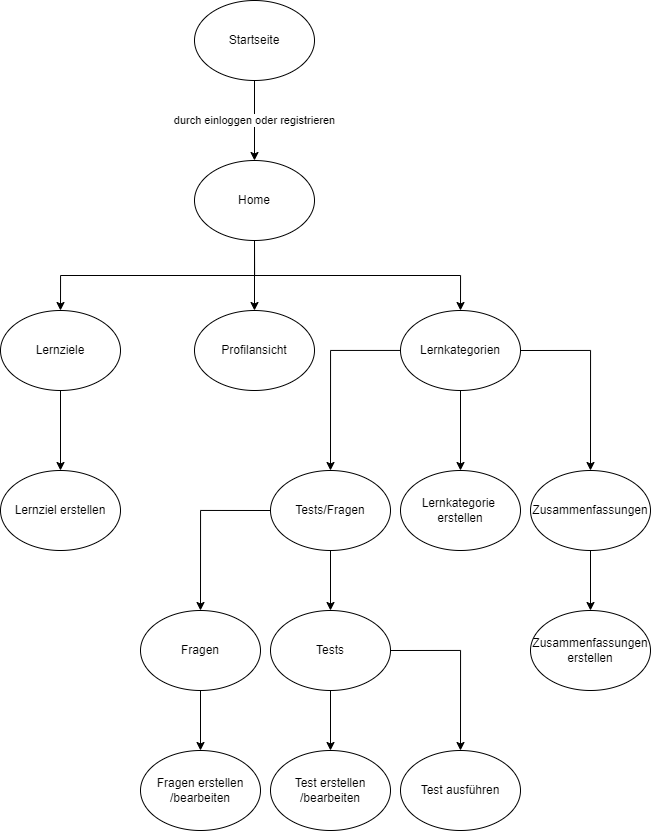
\includegraphics[width=0.8\textwidth]{images/diagramme/Seitenhierarchie.png}
  \caption{Die Seitenhierarchie in LearnAhead}
  \label{fig:UseCaseDiagramm}
\end{figure}

\newpage
\subsubsection{UI-Mockups}

\begin{figure}[htbp]
  \centering
  \begin{subfigure}[b]{0.45\linewidth}
    \centering
    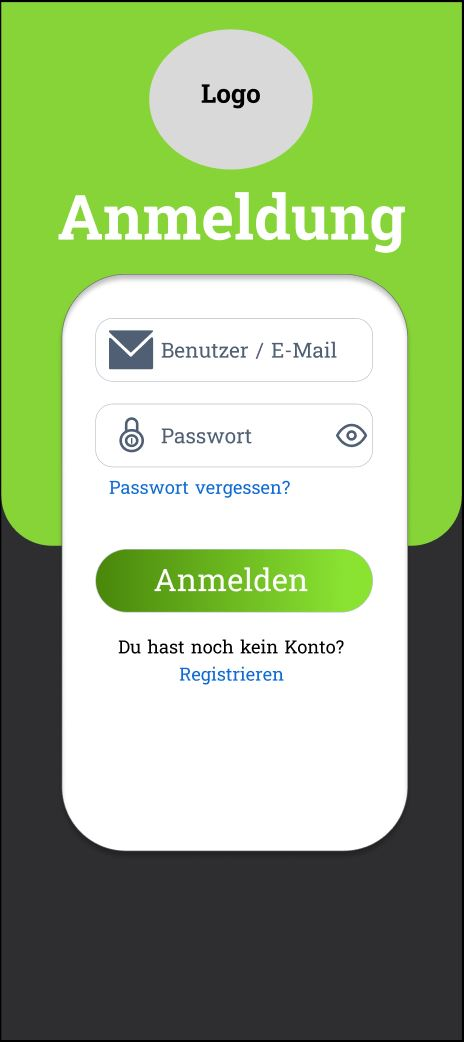
\includegraphics[width=\linewidth]{images/Mockups/Login.JPG}
    \caption{Login-Screen}
    \label{fig:login-screen}
  \end{subfigure}
  \hfill
  \begin{subfigure}[b]{0.45\linewidth}
    \centering
    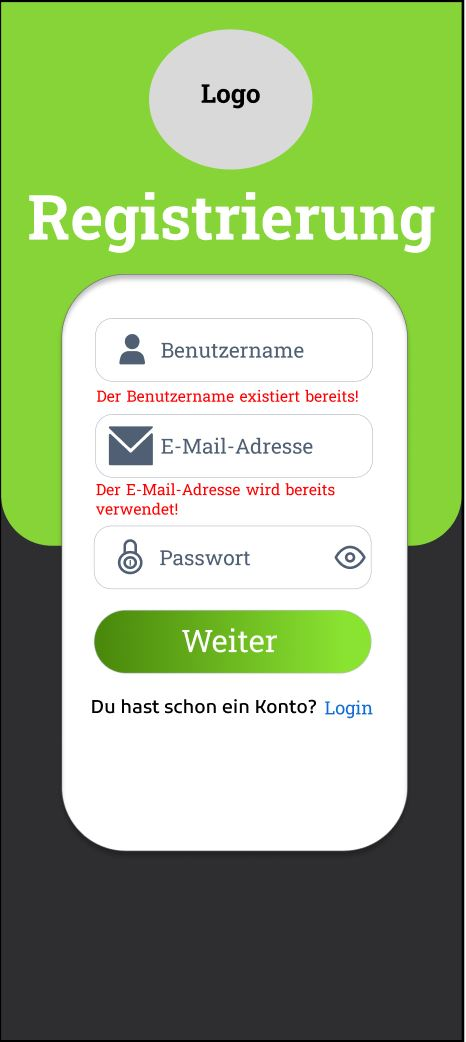
\includegraphics[width=\linewidth]{images/Mockups/Registrierung.JPG}
    \caption{Registrierung}
    \label{fig:registrierung}
  \end{subfigure}
  \caption{Login und Registrierung}
\end{figure}

\newpage

\begin{figure}[htbp]
  \centering
  \begin{subfigure}[b]{0.45\linewidth}
    \centering
    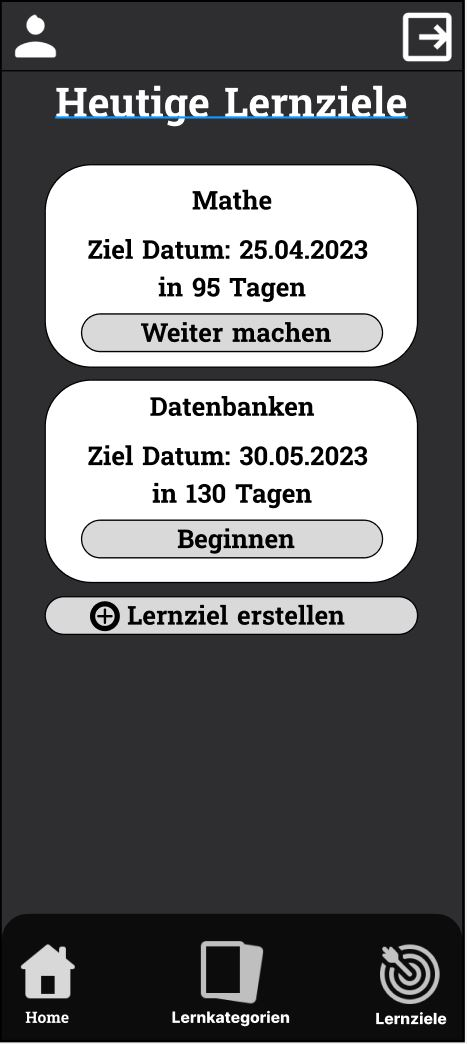
\includegraphics[width=\linewidth]{images/Mockups/Home.JPG}
    \caption{Home-Screen}
    \label{fig:home-screen}
  \end{subfigure}
  \hfill
  \begin{subfigure}[b]{0.45\linewidth}
    \centering
    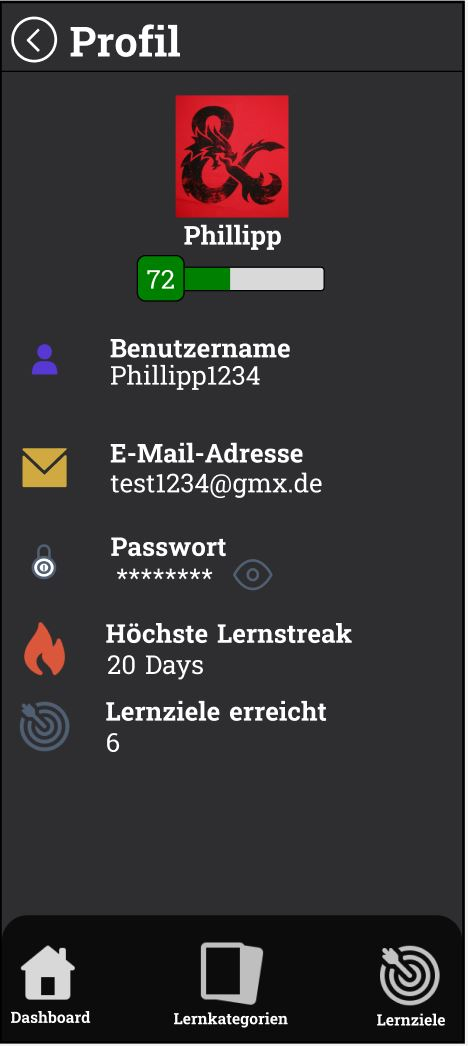
\includegraphics[width=\linewidth]{images/Mockups/Profile.JPG}
    \caption{Profilansicht}
    \label{fig:profilansicht}
  \end{subfigure}
  \caption{Home-Screen and Profilansicht}
\end{figure}

\newpage

\begin{figure}[htbp]
  \centering
  \begin{subfigure}[b]{0.45\linewidth}
    \centering
    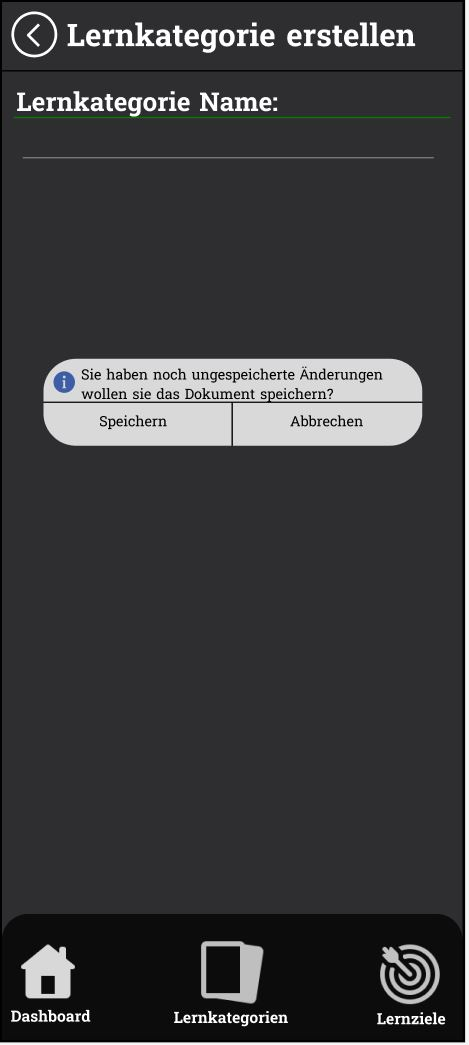
\includegraphics[width=\linewidth]{images/Mockups/createLernkategorie.JPG}
    \caption{Erstellen einer Lernkategorie}
    \label{fig:lernkategorie-create}
  \end{subfigure}
  \hfill
  \begin{subfigure}[b]{0.45\linewidth}
    \centering
    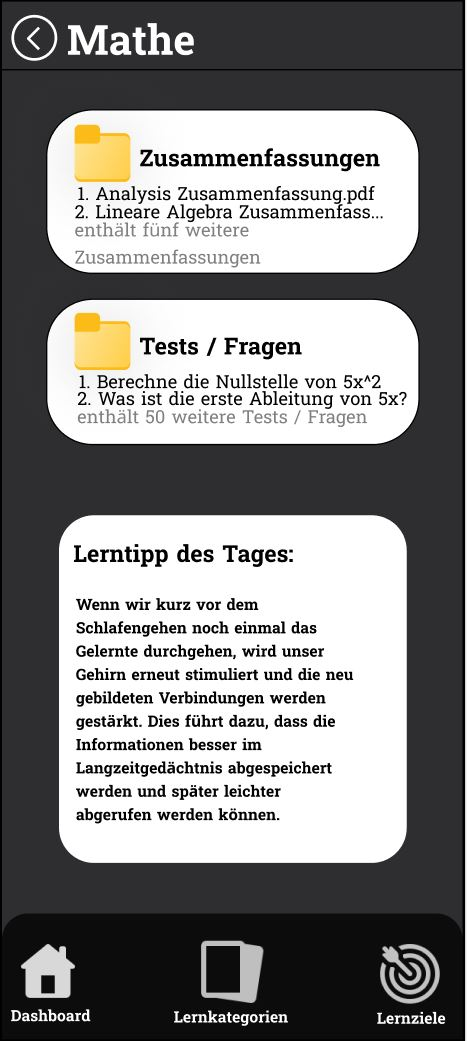
\includegraphics[width=\linewidth]{images/Mockups/Lernkategorie.JPG}
    \caption{Ansicht Lernkategorien}
    \label{fig:lernkategorie-ansicht}
  \end{subfigure}
  \caption{Erstellen einer Lernkategorie and Ansicht Lernkategorien}
  \label{fig:lernkategorie}
\end{figure}

\newpage

\begin{figure}[htbp]
  \centering
  \begin{subfigure}[b]{0.45\linewidth}
    \centering
    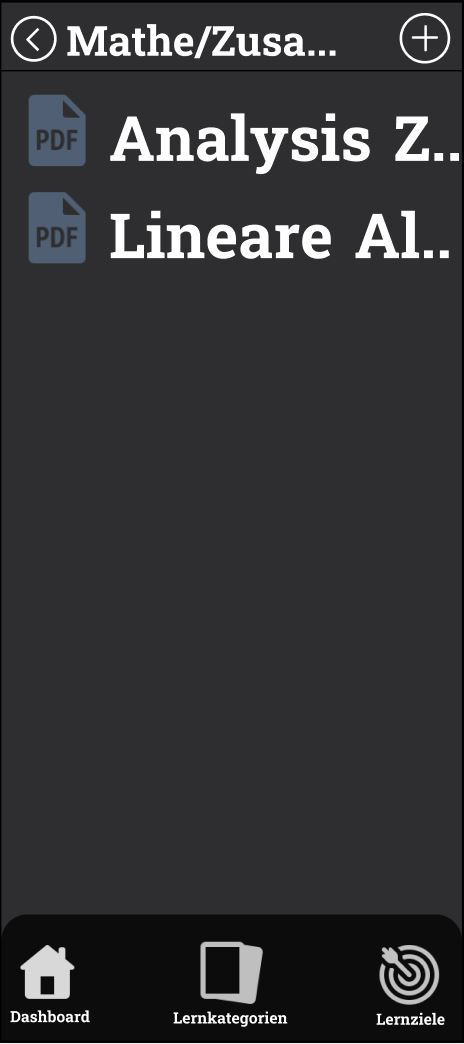
\includegraphics[width=\linewidth]{images/Mockups/Summaries.JPG}
    \caption{Ansicht Zusammenfassungen}
    \label{fig:zusammenfassungen-ansicht}
  \end{subfigure}
  \hfill
  \begin{subfigure}[b]{0.45\linewidth}
    \centering
    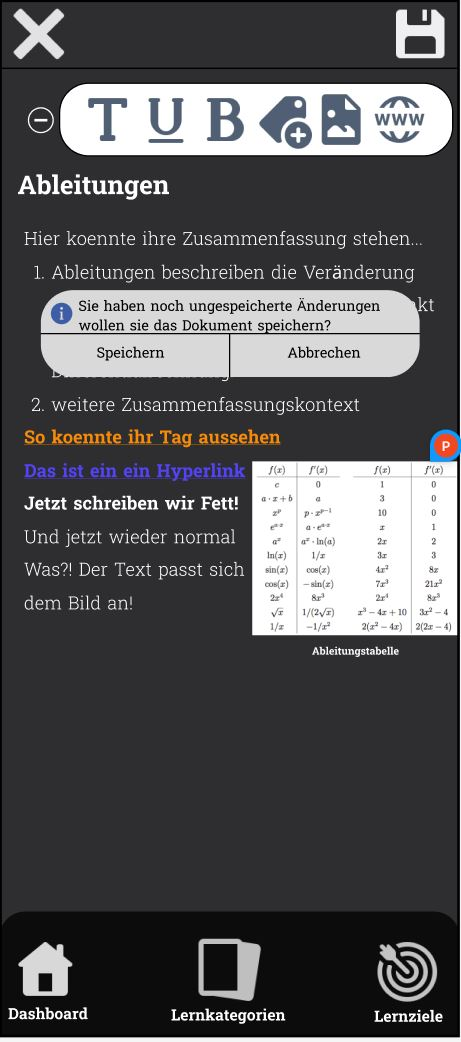
\includegraphics[width=\linewidth]{images/Mockups/Summaries_Look.JPG}
    \caption{Erstellen einer Zusammenfassung}
    \label{fig:zusammenfassungen-erstellen}
  \end{subfigure}
  \caption{Ansicht Zusammenfassungen and Erstellen einer Zusammenfassung}
  \label{fig:zusammenfassungen}
\end{figure}

\newpage

\begin{figure}[htbp]
  \centering
  \begin{subfigure}[b]{0.45\linewidth}
    \centering
    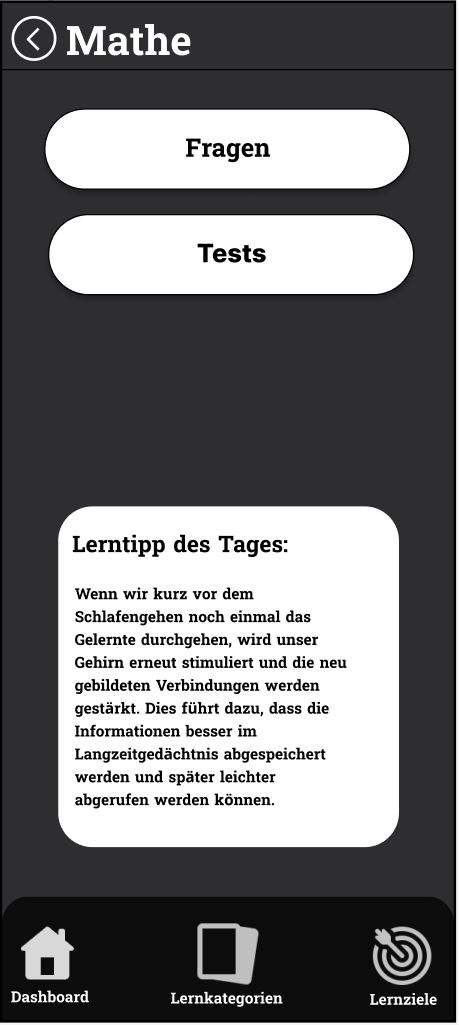
\includegraphics[width=\linewidth]{images/Mockups/FragenTests.JPG}
    \caption{Ansicht Fragen und Tests}
    \label{fig:fragen-tests-ansicht}
  \end{subfigure}
  \hfill
  \begin{subfigure}[b]{0.45\linewidth}
    \centering
    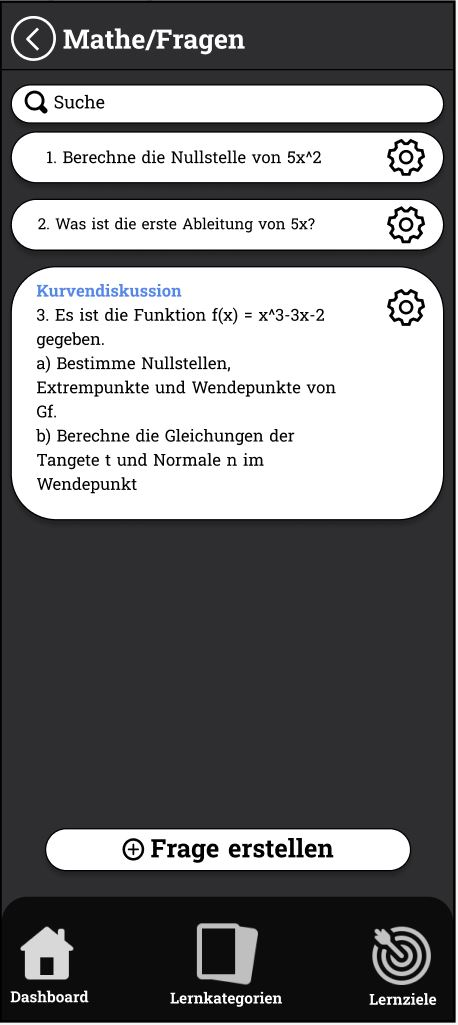
\includegraphics[width=\linewidth]{images/Mockups/Fragen.JPG}
    \caption{Ansicht Fragen}
    \label{fig:fragen-ansicht}
  \end{subfigure}
  \caption{Ansicht Fragen und Tests and Ansicht Fragen}
  \label{fig:fragen-tests}
\end{figure}

\newpage

\begin{figure}[htbp]
  \centering
  \begin{subfigure}[b]{0.45\linewidth}
    \centering
    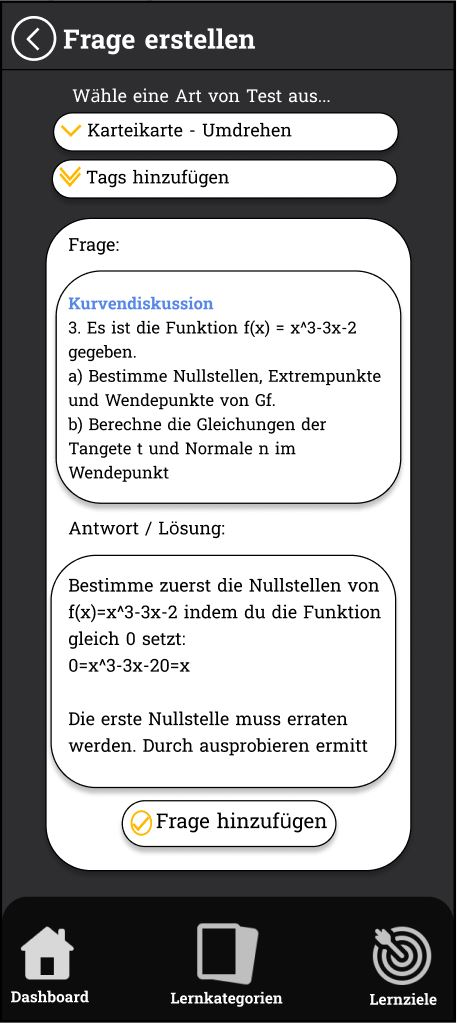
\includegraphics[width=\linewidth]{images/Mockups/FrageErstellen.JPG}
    \caption{Erstellen einer Frage}
    \label{fig:frage-erstellen}
  \end{subfigure}
  \hfill
  \begin{subfigure}[b]{0.45\linewidth}
    \centering
    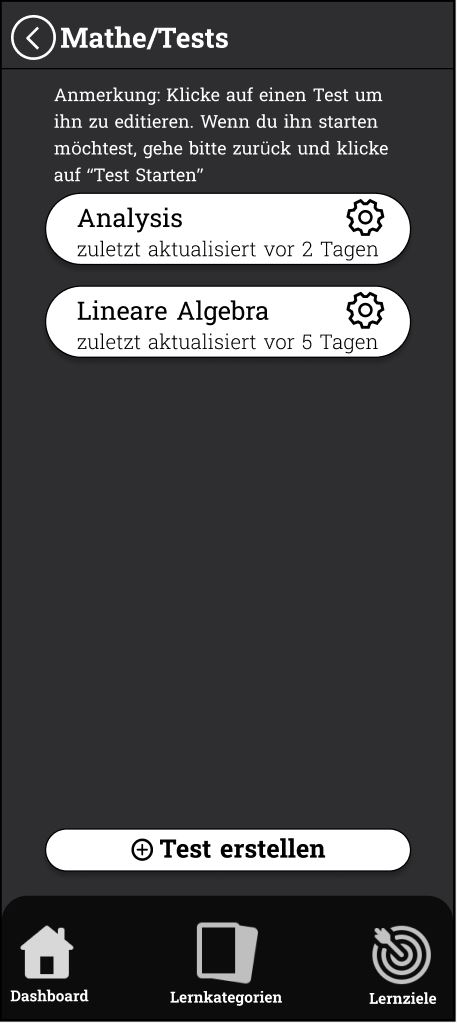
\includegraphics[width=\linewidth]{images/Mockups/Tests.JPG}
    \caption{Ansichts Tests}
    \label{fig:tests-ansicht}
  \end{subfigure}
  \caption{Erstellen einer Frage and Ansichts Tests}
  \label{fig:frage-tests}
\end{figure}

\newpage

\begin{figure}[htbp]
  \centering
  \begin{subfigure}[b]{0.45\linewidth}
    \centering
    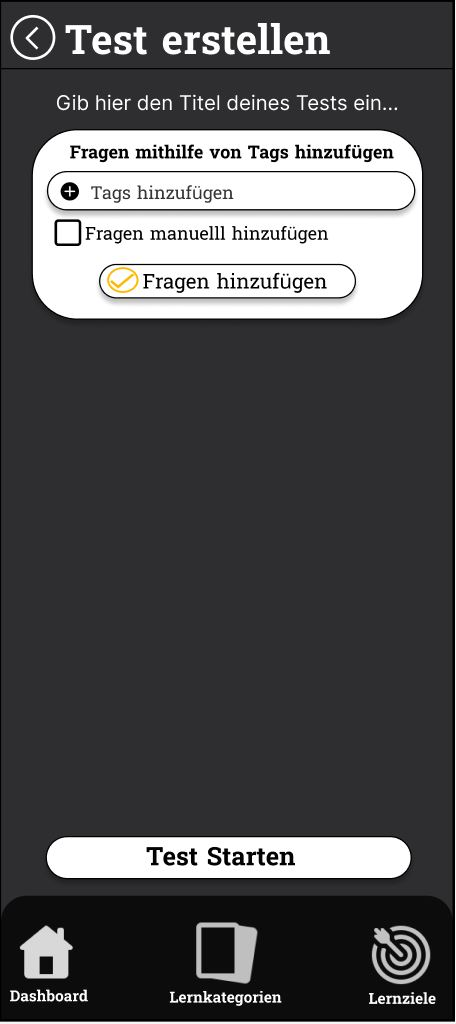
\includegraphics[width=\linewidth]{images/Mockups/TestErstellen.JPG}
    \caption{Erstellen eines Tests}
    \label{fig:test-erstellen}
  \end{subfigure}
  \hfill
  \begin{subfigure}[b]{0.45\linewidth}
    \centering
    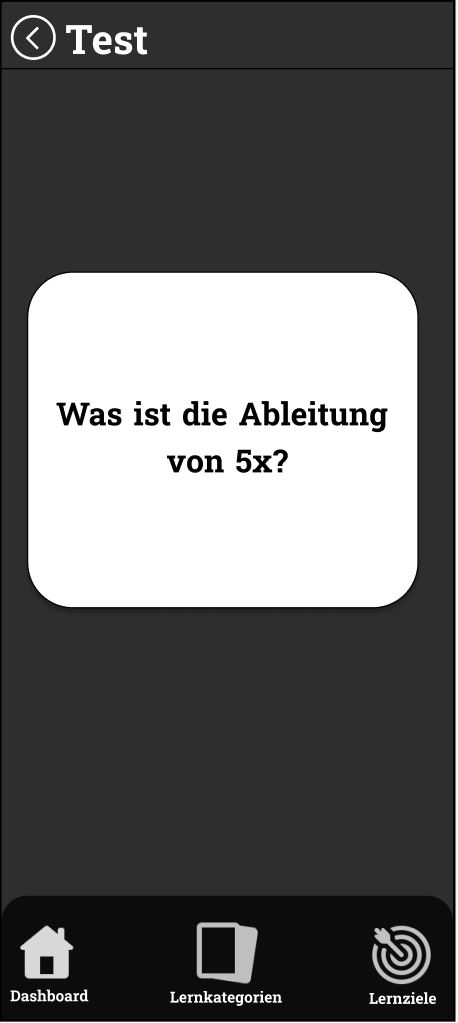
\includegraphics[width=\linewidth]{images/Mockups/TestFrage.JPG}
    \caption{Ansicht einer Frage innerhalb eines Tests}
    \label{fig:test-frage}
  \end{subfigure}
  \caption{Test}
\end{figure}

\newpage

\begin{figure}[htbp]
  \centering
  \begin{subfigure}[b]{0.45\linewidth}
    \centering
    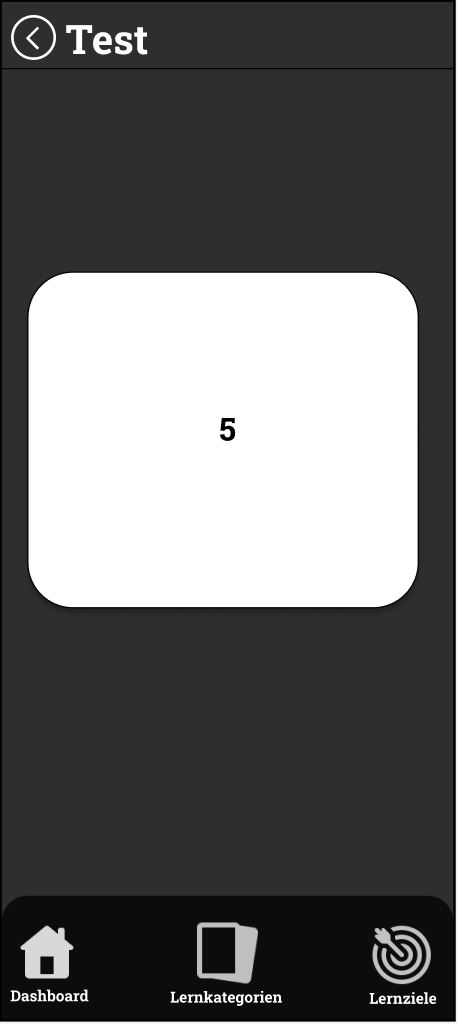
\includegraphics[width=\linewidth]{images/Mockups/TestAntwort.JPG}
    \caption{Ansicht einer Antwort innerhalb eines Tests}
    \label{fig:test-antwort}
  \end{subfigure}
  \hfill
  \begin{subfigure}[b]{0.45\linewidth}
    \centering
    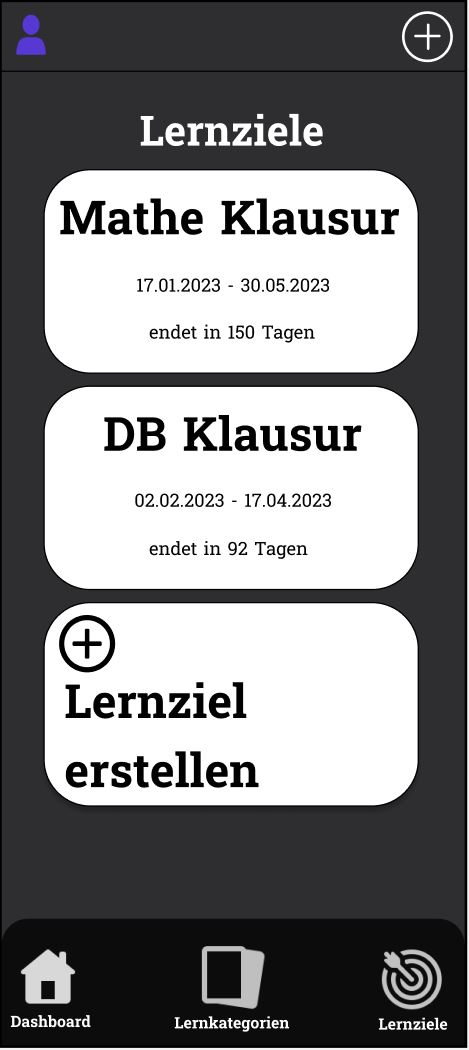
\includegraphics[width=\linewidth]{images/Mockups/Lernziele.JPG}
    \caption{Ansicht Lernziele}
    \label{fig:lernziele}
  \end{subfigure}
  \caption{Test}
\end{figure}

\newpage

\begin{figure}[H]
  \centering
  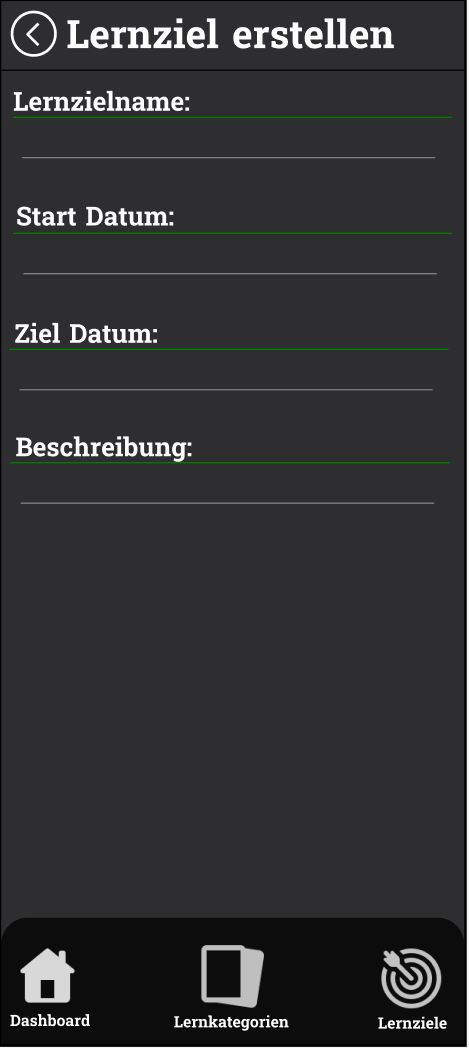
\includegraphics[width=0.5\linewidth]{images/Mockups/LernzielErstellen.JPG}
  \caption{Erstellen eines Lernziels}
  \label{fig:lernziel-erstellen}
\end{figure}

\newpage

\subsection{Datenflussdiagramm}